\chapter{Results and Discussion}

\section{Experiment Summary}

We provide a summary of the $16$ experiments showcased in this work.

\begin{table}[H]
    \scriptsize
    \centering
    \renewcommand{\arraystretch}{1.3}
    \begin{tabularx}{\textwidth}{X c@{\hspace{3em}}c@{\hspace{3em}}c}
        \toprule
        \textbf{Task} & \textbf{Model} & \textbf{Architecture}  & \textbf{Val TIC Macro F1}  \tabularnewline \midrule
        \textbf{A} &
        \begin{tabular}{@{}c@{}}
            Baseline \\ 2-min \\ 8-min \\ 32-min \\ 128-min \\ 4-channel \\ 6-channel \\ \textbf{Chronos-2} \\ Qwen 2.5 0.5B
        \end{tabular} &
        \begin{tabular}{@{}c@{}}
            CNN \\ Transformer \\ Transformer \\ Transformer \\ Transformer \\ Transformer \\ Transformer \\ \textbf{TSFM fine-tune} \\ LLM fine-tune
        \end{tabular} &
        \begin{tabular}{@{}c@{}}
            9061 \\ 0.8396 \\ 0.8704 \\ 0.8684 \\ 0.8436 \\ 0.8931 \\ 0.8983 \\ \textbf{0.9261} \\ 0.9129
        \end{tabular} \tabularnewline \midrule
        \textbf{B} &
        \begin{tabular}{@{}c@{}}
            Baseline \\ 2-min \\ 8-min \\ 32-min \\ 128-min \\ 4-channel \\ 6-channel \\ \textbf{Chronos-2} \\ Qwen 2.5 0.5B
        \end{tabular} &
        \begin{tabular}{@{}c@{}}
            CNN \\ Transformer \\ Transformer \\ Transformer \\ Transformer \\ Transformer \\ Transformer \\ \textbf{TSFM fine-tune} \\ LLM fine-tune
        \end{tabular} &
        \begin{tabular}{@{}c@{}}
            0.9232 \\ 0.6618 \\ 0.8223 \\ 0.8614 \\ 0.9110 \\ 0.9230 \\ 0.9240 \\ \textbf{0.9496} \\ 0.9139
        \end{tabular} \tabularnewline
        \bottomrule
    \end{tabularx}
    \caption[Experiment]{Experiment Summary}
    \label{tab:06_experiment_summary}
\end{table}

\FloatBarrier

As can be seen from \hyperref[tab:06_experiment_summary]{Table 7.1}, the Chronos-2 fine-tunes dominated both tasks, significantly outperforming the other models and was the only model that outperformed the baseline CNN on both tasks.

Because of the low gap between the baseline CNN and the evaluated models that had access to the same training information (all 6 channels enabled), we theorize that the majority of the performance was decided by the multi-channel architecture and light curve segmentation.
The Chronos-2 fine-tune nonetheless consistently beat the CNN which showcased the adaptability of large pretrained transformer models on our task.

\section{Final Model}

Since the Chronos-2 fine-tune performed the best out of all the evaluated configurations, we used it for more experiments, trying to further optimize the hyperparameters specifically for its architecture and achieve better performance.
However, none of the techniques we tried -- increasing dropout, tuning LoRA values, trying different channel combinations and modifying the fusion head -- lead to any improvement over the original experiment.

The original model proposed in \hyperref[subsubsec:06-chronos]{6.9.1 Chronos-2} was therefore chosen as the final best model.
We use the original checkpoints with the best TIC-level Macro F1 (epoch 5 for Task A and epoch 4 for task B) to evaluate the final model's performance on the test set which should simulate new, unknown data.
The model shouldn't be significantly overfitted on either of those checkpoints, since the training validation loss wasn't increasing yet and the training loss was only slightly lower.

\subsection{Task A Test Evaluation and Discussion}

\begin{table}[H]
    \centering
    \footnotesize
    \renewcommand{\arraystretch}{1.1}

    \begin{minipage}[t]{0.32\textwidth}
        \centering
        \begin{tabularx}{\textwidth}{X c}
            \toprule
            \textbf{Metric} & \textbf{Score} \tabularnewline
            \midrule
            Accuracy    &  0.8702 \tabularnewline
            Macro F1    & 0.8693 \tabularnewline
            TIC Accuracy & 0.8946 \tabularnewline
            TIC Macro F1 & 0.8934 \tabularnewline
            \bottomrule
        \end{tabularx}
    \end{minipage}
    \hfill
    \begin{minipage}[t]{0.64\textwidth}
        \centering
        \footnotesize
        \begin{tabularx}{\textwidth}{X c c c c c}
            \toprule
            \textbf{Class} & \textbf{Precision} & \textbf{Recall} & \textbf{F1-score} & \textbf{Support} \tabularnewline
            \midrule
            N & 0.85 & 0.97 & 0.90 & 259 \tabularnewline
            V & 0.96 & 0.82 & 0.88 & 243   \tabularnewline
            \bottomrule
        \end{tabularx}
    \end{minipage}

    \caption[Final Model Test Metrics (A)]{Final Model Test Metrics (Task A)}
    \label{tab:06_final_model_test_metrics_A}
\end{table}

The test TIC-level Macro F1 went down $\approx 0.02$, this can be expected and is a good generalization performance on a dataset of this size.
It should however be noted that for the \textbf{variable} class the precision increased and recall decreased significantly when compared to the validation metrics.

This behavior has interesting implications for real-world use cases -- for example, the model would be really effective in precisely identifying variable stars, that could be utilized to create large datasets consisting of (mostly) variable stars that could be later used for unsupervised pretraining.
However, the downside is that the model will miss out on some potentially interesting variable stars due to its low recall.

\subsection{Task B Test Evaluation and Discussion}

\begin{table}[H]
    \centering
    \footnotesize
    \renewcommand{\arraystretch}{1.1}

    \begin{minipage}[t]{0.32\textwidth}
        \centering
        \begin{tabularx}{\textwidth}{X c}
            \toprule
            \textbf{Metric} & \textbf{Score} \tabularnewline
            \midrule
            Accuracy    &  0.8998 \tabularnewline
            Macro F1    & 0.8340 \tabularnewline
            TIC Accuracy & 0.9333 \tabularnewline
            TIC Macro F1 & 0.8803 \tabularnewline
            \bottomrule
        \end{tabularx}
    \end{minipage}
    \hfill
    \begin{minipage}[t]{0.64\textwidth}
        \centering
        \footnotesize
        \begin{tabularx}{\textwidth}{X c c c c c}
            \toprule
            \textbf{Class} & \textbf{Precision} & \textbf{Recall} & \textbf{F1-score} & \textbf{Support} \tabularnewline
            \midrule
            E & 0.83 & 0.67 & 0.74 & 15 \tabularnewline
            P & 0.94 & 0.99 & 0.96 & 81   \tabularnewline
            R & 0.94 & 0.93 & 0.94 & 39   \tabularnewline
            \bottomrule
        \end{tabularx}
    \end{minipage}

    \caption[Final Model Test Metrics (B)]{Final Model Test Metrics (Task B)}
    \label{tab:06_final_model_test_metrics_B}
\end{table}

The TIC-level Macro F1 dropped significantly ($\Delta \approx 0.07$) compared to the validation set.
Interestingly, the entire drop in performance was caused by the misclassification of $5$ \textbf{eclipsing} stars as another class which lead to greatly decreased recall and eventually Macro F1 score.

We have investigated the 5 misclassified eclipsing stars and found out that each of them was an interesting non-standard example.

\begin{table}[H]
    \centering
    \small
    \renewcommand{\arraystretch}{1.3}
    \begin{tabularx}{\textwidth}{X c X}
        \toprule
        \textbf{TIC} & \textbf{Eclipsing Subclass} & \textbf{Note} \tabularnewline
        \midrule
        224595426 & EA & Extremely noisy, the eclipses are not easily identifiable. \tabularnewline
        229710150 & ELL & Peaks are not sharp -- similar to a rotating star. \tabularnewline
        259238257 & ELL & Peaks are not sharp -- similar to a rotating star. \tabularnewline
        288346083 & EA & Atypically long period -- the eclipse happened only once per 50 days. \tabularnewline
        362226108 & EW & Very similar to a pulsating star. \tabularnewline
        \bottomrule
    \end{tabularx}
    \caption[Missclassified Eclipsing Stars]{Misclassified Eclipsing Stars}
    \label{tab:06_misclassified_eclipsing_stars}
\end{table}

\FloatBarrier

\begin{figure}[!htbp]
    \centering
    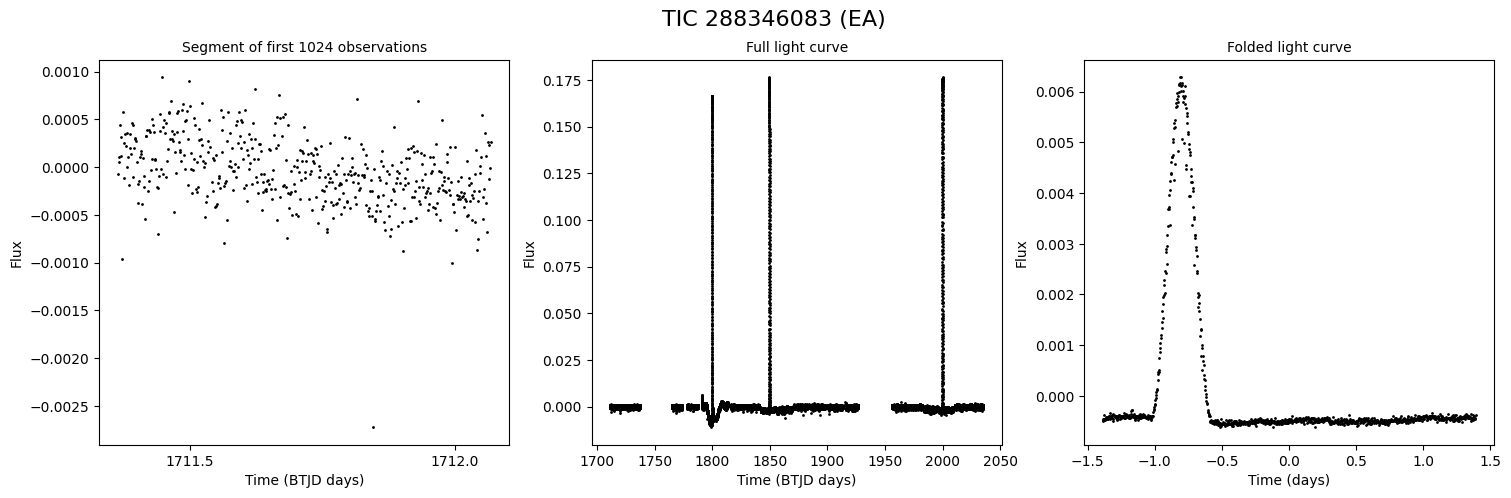
\includegraphics[width=\linewidth]{images/06/long_period_star}
    \caption[Long Period EA Star]{TIC 288346083, a misclassified eclipsing star with atypically long period.}
    \label{fig:06_long_period_star}
\end{figure}

\FloatBarrier

Despite the worse performance on the \textbf{eclipsing} class, the model has generalized well on the remaining 2 classes, their test metrics being nearly identical to the validation metrics.


\section{Computational Performance}

For usage on large real-world datasets, the model must be able to efficiently process large volumes of data (millions of light curves).
We provide a brief analysis of the model's processing speed using available data.

There are 2 main possible bottlenecks:

\begin{itemize}
    \item \textbf{Preprocessing}
    \item \textbf{Inference}
\end{itemize}

\subsection{Preprocessing}

The preprocessing speed was $\approx 13.8 \, \text{light curves/s}$ on AMD Ryzen 5 9700X CPU when utilizing all 8 cores or around \num{1200000} light curves per day.
While the preprocessing pipeline could certainly be optimized, it would probably not achieve more than $10\times$ speedup.

\subsection{Inference}

Information from the training logs shows that model took $10.7$ seconds to run evaluation on the val subset of $135$ light curves, making the inference speed $\approx 12.6 \, \text{light curves/s}$ or around \num{1100000} on an AMD Radeon RX9070 GPU.

\subsection{Summary}

With the available information, we can conclude that the pipeline is theoretically capable of analyzing up to millions of light curves in reasonable time (days) on higher end consumer-grade hardware.
The processing speed could be further increased by utilizing industrial-grade GPU clusters and more parallelization.